\section{Heurística de búsqueda local}
Como vimos en la sección anterior, la heurística golosa no nos provee ninguna garantía de error máximo contra soluciones reales. Una manera de 'amortizar' esto, es realizar optimizaciones por búsqueda local sobre los resultados arrojados por dicha heurística. Dada una instancia de solución al problema y un vecindario definido de otras soluciones, tomamos la vecina de menor distancia total y reiteramos con algún criterio que determine cuándo parar. Si ninguna vecina tenía menor distancia, entonces no es posible ninguna optimización desde esa misma instancia.
\\

Presentaremos dos vecindarios experimentales con el fin de contrastar su rendimiento temporal y sus respectivos errores respecto de la solución real. Al igual que en el caso de la heurística golosa, decidimos basarnos en heurísticas clásicas utilizadas para \emph{TSP}.

\subsection{Búsqueda local por swaps de nodos}
La idea es sencilla: para cualquier par dado de nodos en un camino, supongamos $v$ y $w$ con $w$ recorrido posteriormente a $v$ ¿representa una mejora en la distancia total intercambiarlos de manera que a la hora de visitar $v$ en su lugar recorra $w$ y viceversa?
\\

Así, el vecindario de una solución son todas aquellas resultantes de swapear dos ubicaciones en el vector donde se encuentran por orden.

\subsubsection{Pseudocódigo del algoritmo}

Claramente es necesario recalcalcular la validez de un camino tras swapear dos de sus ubicaciones antes de considerarlo como candidato.

    \begin{lstlisting}
    $\textbf{Def}$ iterar_swap(orden) $\rightarrow\ \langle {float,\ bool} \rangle$

        huboMejora $\gets$ false
        dist $\gets$ distanciaCamino(orden, graph)

        mejor_vecino $\gets$ orden
        $\textbf{Para}$ i $\gets$ 0...|orden|-1:
            $\textbf{Para}$ j $\gets$ i + 1...|orden|-1:
                orden_vecino $\gets$ orden
                orden_vecino[i] $\gets$ orden[j]
                orden_vecino[j] $\gets$ orden[i]

                $\textbf{Para}$ k $\gets$ 0...|orden|-1:
                    $\textbf{Si}$ esGimnasio(orden[k]):
                        ultimo_gim $\gets$ k

                pow $\gets$ 0
                valido $\gets$ esCaminoValido(orden_vecino[0..ultimo_gim], tam_mochila, pow)

                $\textbf{Si}$ $\neg$valido:
                    $\textbf{Proximo j}$

                dist_vecino $\gets$ distanciaCamino(orden_vecino)

                $\textbf{Si}$ dist_vecino < dist:
                    huboMejora $\gets$ true
                    dist $\gets$ dist_vecino
                    mejor_vecino $\gets$ orden_vecino
        orden $\gets$ mejor_vecino
        Retornar $\langle$ dist, huboMejora $\rangle$
    \end{lstlisting}

    Veamos ahora el contexto de búsqueda en que se invoca la función. Recibimos por entrada el orden de recorrido de alguna solución válida desarrollada por la heurística \emph{greedy}, de no ser válida devolvemos un resultado anunciándolo pues no podríamos optimizar una solución inválida, y luego procedemos a insertarle al final todas las paradas que no contenga dicho recorrido. Esto se debe a que, aún cuando no se hayan usado en la solución original, nos interesa maximizar el vecindario de la instancia de modo que podamos explorar la mayor cantidad posible de swapeos. Si la solución que devolveremos no necesita esas paradas para recorrer todos los gimnasios, serán recortadas nuevamente.
    \\

    Un tema de interés respecto a la optimización por búsqueda local es el de escoger la cantidad necesaria de iteraciones a realizar. Por ejemplo, una opción sería iterar hasta que no se encuentre ninguna mejora en el último vecindario. Si bien maximiza posibilidades de encontrar una buena solución, es potencialmente costosa dado que si en cada llamado a $iterar_swap$ encontramos una nueva mejor solución podría llegar a ser necesario mejorar cada una de las permutaciones posibles del arreglo de ubicaciones (de cardinal factorial en su longitud) en un supuesto peor caso. Por lo tanto, buscando un comportamiento polinómico, iteramos una cantidad fija de veces de acuerdo a un parámetro de entrada (corridas). Si corridas es 0 se itera como describimos antes, hasta que no haya mejoras, de lo contrario se itera $corridas$ veces o hasta llegar a un vecindario sin mejores soluciones.

    \begin{lstlisting}
    $\textbf{Def}$ local_swap(orden, corridas) $\rightarrow \langle {float,\ int,\ vector} \rangle$

        $\textbf{Si}$ |orden| = 0:
            $\textbf{Retornar}$ $\langle$ $\infty$, 0, [] $\rangle$

        usada $\gets$ [nstops] $\times$ (false)        $\emph{// usada = [false.. false]}$
        $\textbf{Para}$ i en orden:
            $\textbf{Si}$ i $\geq$ #gimnasios:
                usada[i - #gimnasios] $\gets$ true

        $\textbf{Para}$ parada $\gets$ 0..#paradas:
            Si $\neg$usada[parada]:
                orden $\gets$ orden ++ [parada + #gimnasios]

        seguir $\gets$ true
        $\textbf{Mientras}$ seguir:
            ult_corrida $\gets$ iterar_swap(orden);
            seguir $\gets$ ult_corrida.second
            dist $\gets$ ult_corrida.first
            $\textbf{Si}$ corridas > 0:
                corridas $\gets$ corridas - 1
                seguir $\gets$ (seguir $\land$ (corridas > 0))

        $\textbf{Para}$ k $\gets$ 0...|orden|-1:
            $\textbf{Si}$ esGimnasio(orden[k]):
                ultimo_gim $\gets$ k

        orden $\gets$ orden[0..ultimo_gim]

        $\textbf{Retornar}$ $\langle$ dist, |orden|, orden $\rangle$
    \end{lstlisting}

\subsubsection{Complejidad del algoritmo}
    Empecemos por calcular la complejidad de $iterar\_swap$. Arranca calculando la distancia del camino conformado por $orden$ con un costo de $\mathcal{O}(|orden|)$ que es $\mathcal{O}(\#gimnasios + \#paradas)$ considerando que se rellenan todas las paradas faltantes desde $local\_swap$. Luego se copia el contenido de $orden$ a $mejor\_vecino$, en $\mathcal{O}(\#gimnasios + \#paradas)$ en el mismo peor caso que ya mencionamos.
    \\

    Luego se ejecuta un ciclo que itera $\mathcal{O}((\#gimnasios + \#paradas)^2)$ veces.
    \\

    Dentro del ciclo se hace una copia de $orden$ en $\mathcal{O}(\#gimnasios + \#paradas)$, se hace el swap de ubicaciones en $\mathcal{O}(1)$ (asignar índices de nodos en un vector es constante), se busca el índice del gimnasio en $\mathcal{O}(\#gimnasios + \#paradas)$ \footnote{Como ya ha sucedido en otras secciones se aclara que en nuestra implementación algunas operaciones como esta se realizan sobre iteradores pero se usan versiones sobre índices equivalentes en complejidad por simplicidad de lectura de pseudocódigo.}. Luego, se calcula si el camino nuevo es válido con costo $\mathcal{O}(\#gimnasios + \#paradas)$ peor caso (que el último gimnasio sea la última ubicación del arreglo de órdenes), se calcula también su longitud hasta el último gimnasio, de ser válido el camino, en $\mathcal{O}(\#gimnasios + \#paradas)$ y por último se actualizan las variables que guardan los mejores resultados vistos hasta el momento en $\mathcal{O}(\#gimnasios + \#paradas)$, costo correspondiente al copiado de $orden\_vecino$ en el peor caso de contener todas las paradas además de gimnasios.
    \\

    Por lo tanto tenemos un costo total del ciclo de $\mathcal{O}((\#gimnasios + \#paradas)^3)$. Que se corresponde también con el costo total de la función considerando que absorbe los costos del primer cálculo de distancia y asignar a $orden$ la mejor solución hallada (ambos lineales en el tamaño de orden).
    \\

    Para $local\_swap$ empezamos corroborando que $orden$ sea una secuencia de tamaño mayor que 0 y retornando un valor específico en $\mathcal{O}(1)$. Inicializamos el vector de $bool$ sobre paradas usadas en $\mathcal{O}((\#paradas))$ y luego se marcan en $\mathcal{O}(|orden|)$, que en peor caso es $\mathcal{O}(\#gimnasios + \#paradas)$ por contener todas las ubicaciones, para después agregar en $\mathcal{O}(1)$ todas las paradas recorridas linealmente que no estén usadas ($\mathcal{O}(\#paradas)$).
    \\

    Para el ciclo que convoca a $iterar\_swap$ aparte del llamado a esta función solamente realizamos asignaciones y comparaciones numérico-booleanas, por lo que prepondera la complejidad de $iterar\_swap$ que es, como vimos antes, cúbica en la cantidad total de ubicaciones.
    \\

    Como la cantidad de veces que ejecuta el ciclo depende de si $corridas$ es mayor a 0 o igual, se separan dos casos: ejecutar el ciclo $corridas$ veces o ejecutar hasta que no se encuentren mejoras. Este último caso resulta ser de orden factorial hipotetizando algún peor caso en el que se realice una actualización (produciendo mejora) por cada permutación posible de $orden$. Aún si en cada llamado a $iterar\_swap$ cubrimos la cuota superior de mejorar un orden cuadrático de veces, aún faltaría hacer $\mathcal{O}((\#gimnasios + \#paradas)!/(\#gimnasios + \#paradas)^2) = \mathcal{O} ((\#gimnasios + \#paradas)!)$ llamados hasta dejar de ver mejoras.
    \\

    El ciclo entonces queda, con complejidad $\mathcal{O}(corridas*(\#gimnasios + \#paradas)^3)$ si $corridas > 0$, o $\mathcal{O}((\#gimnasios + \#paradas)!*(\#gimnasios + \#paradas)^3) = \mathcal{O}((\#gimnasios + \#paradas)!)$ si se debe iterar hasta dejar de ver mejoras. En ambos casos la complejidad de ubicar linealmente el índice del último gimnasio y recortar $orden$ es, en peor caso, $\mathcal{O}(\#gimnasios + \#paradas)$.
    \\

    Por lo tanto, sumando todas las complejidades, donde preponderan las del ciclo, queda $\mathcal{O}(corridas*(\#gimnasios + \#paradas)^3)$ si $corridas > 0$, o $\mathcal{O}((\#gimnasios + \#paradas)!)$ si $corridas = 0$. Esta última cota parecería indicar que iterar de esta manera sería similar en costo a la del backtracking o fuerza bruta, pero previo a realizar experimentaciones podemos especular con que realmente no sucedan por lo general casos donde se prolongue significativamente el hallazgo continuo de mejoras. Más adelante contrastaremos empíricamente si esto efectivamente es así.

    \subsubsection{Variación alternativa del algoritmo}
    Originalmente la idea que se nos había ocurrido era, en vez de tomar el mejor de los vecinos de la instancia en cada iteración, tomar el primer vecino que fuera mejor que el actual y seguir luego sin repetir pares $(i,j)$ aún tras haber actualizado la instancia sobre la cual se itera su vecindario.
    \\

    Es decir, cada vez que vemos una solución que mejore a la actual, la pisamos y seguimos con los pares $(i,j)$ restantes. Esto último se debe a que si volvieramos a tomarlos desde $(0,0)$ cada vez que se actualiza la solución, caeríamos en una situación similar a la del peor caso con $corridas = 0$ del algoritmo anterior donde potencialmente se recorrían todas las permutaciones (incluso cuando $corridas$ fuera distinta de 0).
    \\

    Al no repetir pares $(i,j)$ dentro de un mismo llamado y siendo el código extremadamente similar (en vez de actualizar $mejor\_vecino$ se pisa $orden$ con $orden\_vecino$) la complejidad se mantiene igual que en la subsección anterior. Por los motivos anteriores no se considera necesario repetir el pseudocódigo.
    \\

    Aunque no tome necesariamente el mínimo de los vecinos como sí lo hace la implementación que mostramos anteriormente, nos interesó la cuestión de, si al tomar siempre la primer solución 'buena' de cada vecindario y pudiendo actualizar más de una solución por llamado a $iterar\_swap$, se produjeran mejoras en rendimiento. Esto lo pondremos a prueba en la sección de experimentación.

    \subsection{Búsqueda local por 2opt}

    Dado un camino, ¿existen dos pares continuos de ubicaciones $(orden_i,\ orden_{i+1})$ y $(orden_k,\ orden_{k+1})$ tal que $distancia(orden_i,\ orden_{i+1})$ + $distancia(orden_k,\ orden_{k+1}) \ < \ distancia(orden_i,\ orden_k)$ + $distancia(orden_{i+1},\ orden_{k+1})$?
    \\

    De ser así, podemos 'swapear' las aristas $(orden_i,\ orden_{i+1})$ y $(orden_k,\ orden_{k+1})$ por $(orden_i,\ orden_k)$ y $(orden_{i+1},\ orden_{k+1})$ obteniendo un camino de mejor longitud aunque no sea necesariamente válido, por lo que haría falta corroborar su validez. Esta estrategia se llama $2opt$ \footnote{https://en.wikipedia.org/wiki/2-opt} y es un caso particular de la heurística \emph{Lin–Kernighan} \footnote{https://en.wikipedia.org/wiki/Lin-Kernighan_heuristic} usada generalmente para \emph{TSP}.
    \\

    Cabe destacar que en grafos dirigidos esto implicaría recorrer en sentido inverso $orden[i+1..k]$, lo cual no afecta la distancia del subcamino. Entonces nos alcanza con realizar la transformación $orden \gets orden[0..i] ++ reverso(orden[i+1..k]) ++ orden[k+1..|orden|-1]$ para realizar el swap de aristas deseado.

    \begin{figure}[H]
        \centering
        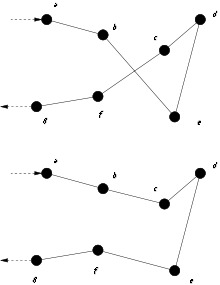
\includegraphics[height=8cm]{2opt}
        \caption{Sea $(b,e)$ la arista $(orden_i,\ orden_{i+1})$ de nuestro ejemplo y $(c,f)$ nuestra $(orden_k,\ orden_{k+1})$, se puede apreciar que se recorre de manera reversa $orden[i+1..k]$ = $[e,d,c]$ tras el swap 2opt.}
        \label{fig:2opt}
    \end{figure}

    Definimos entonces el vecindario de una solución para esta heurística como todas aquellas secuencias de ubicaciones resultantes de invertir una subsecuencia.

    \newpage
    \subsubsection{Pseudocódigo del algoritmo}

    \begin{lstlisting}
    $\textbf{Def}$ iterar2opt(orden, verbose) $\rightarrow$ $\langle {float,\ bool} \rangle$:

        dist $\gets$ distanciaCamino(orden)

        huboMejora $\gets$ false

        $\textbf{Para}$ i $\gets$ 0..|orden|-1:
            $\textbf{Para}$ j $\gets$ i + 1..orden.size()-1:
                orden_vecino $\gets$ orden[0..i] ++ reverso(orden[i+1..j]) ++ orden[j+1..|orden|-1]

                $\textbf{Para}$ k $\gets$ 0...|orden|-1:
                    $\textbf{Si}$ esGimnasio(orden[k]):
                        ultimo_gim $\gets$ k

                pow $\gets$ 0
                valido $\gets$ esCaminoValido(orden_vecino[0..ultimo_gim], tam_mochila, pow)

                $\textbf{Si}$ $\neg$valido:
                    $\textbf{Proximo j}$

                dist_vecino $\gets$ distanciaCamino(orden_vecino)

                $\textbf{Si}$ dist_vecino < dist:
                    huboMejora $\gets$ true
                    dist $\gets$ dist_vecino
                    orden $\gets$ orden_vecino
        Retornar $\langle$ dist, huboMejora $\rangle$
    \end{lstlisting}
